% ==============================================================================
% Paper O1 -- Projective Resolution Dynamics on Variable-Valence Relaxation Graphs
% Complete compilable document
% ==============================================================================

\documentclass[11pt]{article}

\usepackage{amsmath,amssymb,amsthm}
\usepackage{geometry}
\usepackage{hyperref}
\usepackage{graphicx}
\usepackage{cite}
\usepackage{doi}

\geometry{margin=1in}

% -- theorem environments ------------------------------------------------------
\newtheorem{theorem}{Theorem}[section]
\newtheorem{proposition}[theorem]{Proposition}
\newtheorem{corollary}[theorem]{Corollary}
\newtheorem{definition}[theorem]{Definition}
\newtheorem{remark}[theorem]{Remark}

% -- theorem environments without numbering (for informal statements) ----------
\newtheorem*{theorem*}{Theorem}
\newtheorem*{proposition*}{Proposition}
\newtheorem*{corollary*}{Corollary}

% -- macros --------------------------------------------------------------------
\newcommand{\Lproj}{\Lambda_{\mathrm{proj}}}
\newcommand{\lADE}[1]{\lambda_{#1}^{\mathrm{ADE}}}
\newcommand{\widthKM}{\mathrm{width}_{\mathrm{KM}}}
\newcommand{\FKM}{F_{\mathrm{KM}}}
\newcommand{\rKM}{\rho_{\mathrm{KM}}}

% -- metadata ------------------------------------------------------------------
\title{Projective Resolution Dynamics on Variable-Valence Relaxation Graphs}

\author{J\'er\^ome Beau}

\date{\today}

\begin{document}

  \maketitle

  \begin{abstract}
    The spectral relaxation programme recently identified an asymptotic saturation
    of the projective resolution threshold $\Lproj$ for LPS relaxation graphs at
    fixed valence, leading to a structural inversion in the ordering of ADE
    stratigraphic levels.
    In this paper we show that this saturation is not intrinsic to the relational
    substrate but an artefact of holding the LPS parameter $p$ constant.
    Allowing the valence to grow along the cascade causes the Kesten--McKay
    spectral support to contract towards its midpoint, which forces the ADE levels
    to exit the support in a fixed order determined solely by their distance from
    the midpoint.
    This restores a non-trivial dynamical regime for $\Lproj$ and yields the
    effective mass ordering $M_3 > M_1 > M_2$, correcting the fixed-valence
    inversion through a purely geometric mechanism.
    The correction is independent of the precise growth law $p(n) \to \infty$.
    The quantitative amplitude of the inter-generational hierarchy is not addressed
    here and is left to subsequent work combining the present mechanism with the
    hierarchical cascade or sub-linear energy-rank structures identified in the
    companion paper.

    \medskip
    \noindent\textbf{Keywords:}
    projective resolution, relaxation graphs, Ramanujan graphs, LPS graphs,
Kesten--McKay law, spectral gap, Cheeger inequality, variable valence,
spectral stratigraphy, mass hierarchy
  \end{abstract}

  \clearpage
  \tableofcontents

  \clearpage
  \section{Introduction}
    \label{sec:intro}

    \subsection{Context and motivation}
      \label{subsec:context}

      The admissibility sub-programme of Cosmochrony~\cite{cosmochrony} aims to
      derive the number and mass hierarchy of
      particle generations from purely spectral and relational data.
      The programme proceeds through a sequence of companion papers, each
      establishing one structural layer: spectral admissibility~\cite{Beau2026a1},
      spectral capacity~\cite{Beau2026a2}, Gram rigidity~\cite{Beau2026a3}, spectral
      stratigraphy~\cite{Beau2026a4}, and asymptotic saturation~\cite{Beau2026a5}.

      The paper~\cite{Beau2026a4} establishes that the representation-theoretic
      structure of ADE binary Cayley graphs fixes the number of stratigraphic
      levels at three and determines their topological order, while the dynamical
      growth of the projective resolution threshold $\Lproj(n)$ controls their
      separation.
      The paper~\cite{Beau2026a5} analyses this second question.
      Its main positive results include the isoperimetric law
      $\Lproj(n) \asymp h(G(n))^2$, the Cheeger enclosure
      $\lambda_2^2/2 \lesssim \Lproj \lesssim \lambda_2$, and the linear growth
      law $N(\lambda;\,n) \sim \FKM(\lambda) \cdot n$ for the LPS family at fixed
      valence.

      However, \cite{Beau2026a5} also identifies two structural limitations of the
      fixed-valence regime.
      First, the spectral gap $\lambda_2(n)$ converges to the lower edge of the
      Kesten--McKay support as $q \to \infty$ at fixed $p$, causing $\Lproj(n)$ to
      saturate asymptotically; the relaxation cascade then reaches a spectrally
      stationary regime, incapable of generating a viable inter-generational
      hierarchy.
      Second, the effective mass ordering predicted by the fixed-valence saturation
      mechanism inverts the ordering required by the admissibility envelope
      of~\cite{Beau2026a4}.
      Both limitations are traced to a single cause: holding the LPS parameter $p$
      constant.

    \subsection{Main results}
      \label{subsec:results}

      This paper studies the regime in which $p$ grows with the cascade depth $n$,
      defining what we call \emph{variable-valence LPS sequences}
      (Definition~\ref{def:vv_sequence}).
      The three main results are the following.

      \begin{proposition*}[KM contraction, informal]
  Along any variable-valence LPS sequence, the Kesten--McKay support width
  satisfies
  \[
    \widthKM(p(n)) \;=\; \frac{4\sqrt{p(n)}}{p(n)+1} \;\longrightarrow\; 0,
  \]
  with both support edges converging to the midpoint $\lambda = 1$ at rate
  $2/\sqrt{p(n)}$.
      \end{proposition*}

      \begin{theorem*}[ADE exit order, informal]
  For the $2I$ group with the order-5 generating set, the three ADE eigenvalue
  levels exit the contracting Kesten--McKay support in a fixed order:
  \begin{enumerate}
    \item $\lADE{3} = 5/4$ exits first, at the critical prime
    $p_3^* = (4 + \sqrt{15})^2 \approx 62$;
    \item $\lADE{1} = 5/6$ exits second, at $p_1^* = (6 + \sqrt{35})^2
    \approx 142$;
    \item $\lADE{2} = 1$ never exits for any finite $p$.
  \end{enumerate}
  This exit order is a structural consequence of the support geometry,
  independent of the precise growth law $p(n) \to \infty$.
      \end{theorem*}

      \begin{corollary*}[Restored dynamics, informal]
  The Ramanujan lower bound controlling $\lambda_2(n)$ increases along any
  variable-valence LPS sequence, removing the fixed-valence saturation plateau
  and yielding the effective mass ordering $M_3 > M_1 > M_2$.
  This corrects the effective mass ordering inversion of~\cite{Beau2026a5}
  by a geometric mechanism.
      \end{corollary*}

      The formal statements and proofs appear in
      Sections~\ref{sec:variable_valence}--\ref{sec:mass_ordering}.

    \subsection{What this paper does not prove}
      \label{subsec:non_results}

      In the interest of precision, we state explicitly what lies outside the scope
      of the present paper.

      The amplitude of the inter-generational effective mass ratios is not
      determined.
      The variable-valence mechanism removes the structural obstruction to generating
      ratios of order $10^{-4}$--$10^{-5}$, but a quantitative derivation requires
      combining direction (O1) with the hierarchical cascade of direction (O2) or
      the sub-linear energy-rank relation of direction (O3)
      (cf.~\cite{Beau2026a5}, Section~6.5).

      The level-to-generation map is not established from first principles.
      The ordering $M_3 > M_1 > M_2$ is derived structurally; its identification
      with specific Standard Model generations requires additional input
      from~\cite{Beau2026a4} and is left open here.

      The Ramanujan property is used only through the lower
      bound~\eqref{eq:ramanujan_lower}.
      No claim is made about the convergence of $\lambda_2(n)$ itself; only the
      behaviour of the lower bound $\lambda_-(p(n))$ is controlled.

    \subsection{Organisation}
      \label{subsec:organisation}

      Section~\ref{sec:background} collects the necessary definitions and results
      from the admissibility sub-programme.
      Section~\ref{sec:saturation} summarises what~\cite{Beau2026a5} established and
      isolates the root cause of the fixed-valence limitations.
      Section~\ref{sec:variable_valence} introduces the variable-valence LPS family
      and proves the KM contraction and the ADE exit order theorem.
      Section~\ref{sec:mass_ordering} derives the effective mass ordering and
      corrects the fixed-valence inversion.
      Section~\ref{sec:amplitude} analyses the amplitude problem, establishing what
      is resolved and what remains open.
      Section~\ref{sec:physical} provides the physical interpretation in the Cosmochrony
      framework.
      Section~\ref{sec:conclusion} states the conclusions and open directions.

  \section{Background: Projective Resolution and the Relaxation Cascade}
    \label{sec:background}


    We collect the definitions and results from the admissibility sub-programme
    that are used throughout this paper.
    All notation follows~\cite{Beau2026a5}.

    \subsection{Relational substrate and relaxation graphs}
      \label{subsec:graphs}

      Fix a prime $p \equiv 1 \pmod{4}$ and a prime $q \equiv 1 \pmod{4}$ with
      $p \neq q$.
      The \emph{LPS relaxation graph} at parameter $p$ is the Cayley graph
      \begin{equation}
        G = X^{p,q},
      \end{equation}
      whose vertex set is $\mathrm{PSL}(2,\mathbb{F}_q)$, of order
      $\tfrac{1}{2}q(q^2-1)$, and whose valence is
      \begin{equation}
        d = p + 1.
      \end{equation}
      By construction, $X^{p,q}$ is $(p+1)$-regular and Ramanujan for every
      admissible pair $(p,q)$~\cite{LPS}.

      We work throughout with the \emph{normalised Laplacian}
      $\mathcal{L} = I - A/d$, whose eigenvalues lie in $[0,2]$ and are ordered as
      $0 = \lambda_1 \leq \lambda_2 \leq \cdots$.
      In this normalisation the Ramanujan bound reads
      \begin{equation}
        \lambda_2 \;\geq\; 1 - \frac{2\sqrt{p}}{p+1},
        \label{eq:ramanujan_lower}
      \end{equation}
      with the lower bound attained asymptotically along subsequences of the LPS
      family~\cite{LPS}.

    \subsection{Projective resolution}
      \label{subsec:lambda_proj}

      Following~\cite{Beau2026a5}, the \emph{projective resolution threshold}
      $\Lproj(n)$ associated with a sequence of relaxation graphs $G(n)$ of
      increasing size $n$ is defined via the isoperimetric constant:
      \begin{equation}
        \Lproj(n) \;\asymp\; h(G(n))^2,
        \label{eq:lambda_proj_def}
      \end{equation}
      where $h(G)$ denotes the edge-isoperimetric (Cheeger) constant of $G$.
      The Cheeger inequalities give a two-sided control by $\lambda_2$:
      \begin{equation}
        \frac{\lambda_2(n)^2}{2} \;\lesssim\; \Lproj(n) \;\lesssim\; \lambda_2(n).
        \label{eq:cheeger}
      \end{equation}
      Equation~\eqref{eq:cheeger} shows that the entire dynamics of $\Lproj(n)$
      is controlled by the behaviour of the spectral gap $\lambda_2(n)$.
      This reduction from isoperimetric to spectral language is the key technical
      simplification used throughout this paper.

    \subsection{Kesten--McKay spectral density}
      \label{subsec:km}

      For an infinite $d$-regular tree (and hence asymptotically for $d$-regular
      expanders), the \emph{Kesten--McKay measure}~\cite{McKay,Kesten} is the
      probability measure on $[0,2]$ with density
      \begin{equation}
        \rKM(\lambda;\,d) \;=\;
        \frac{d\sqrt{4(d-1) - (d\lambda - d)^2}}{2\pi\,[\,d^2 - (d\lambda - d)^2\,]},
        \qquad \lambda \in [\lambda_-(d),\,\lambda_+(d)],
        \label{eq:KM_density}
      \end{equation}
      where the support edges are, in the LPS parametrisation $d = p+1$,
      \begin{equation}
        \lambda_\pm(p) \;=\; 1 \pm \frac{2\sqrt{p}}{p+1}.
        \label{eq:KM_support_p}
      \end{equation}
      Since the term $d(\lambda - 1)$ appears only squared in~\eqref{eq:KM_density},
      the density is symmetric about $\lambda = 1$:
      \begin{equation}
        \rKM(\lambda) \;=\; \rKM(2 - \lambda),
        \label{eq:KM_symmetry}
      \end{equation}
      and in particular the support satisfies
      \begin{equation}
        \lambda_-(p) \;=\; 2 - \lambda_+(p).
        \label{eq:support_symmetry}
      \end{equation}
      The \emph{Kesten--McKay window width} is
      \begin{equation}
        \widthKM(p) \;:=\; \lambda_+(p) - \lambda_-(p) \;=\; \frac{4\sqrt{p}}{p+1},
        \label{eq:KM_width}
      \end{equation}
      which scales as $4/\sqrt{p}$ for large $p$.
      This rate of contraction is the driving mechanism studied in
      Section~\ref{sec:variable_valence}.

    \subsection{ADE eigenvalue levels}
      \label{subsec:ADE}

      The spectral stratigraphic structure of the admissibility programme is indexed
      by the ADE binary groups~\cite{Beau2026a4}.
      For the binary icosahedral group $2I$ with the order-5 generating set
      $|S| = 24$, the normalised Laplacian has three distinct non-trivial eigenvalue
      levels~\cite{Beau2026a5}:
      \begin{equation}
        \lADE{1} \;=\; \tfrac{5}{6}, \qquad
        \lADE{2} \;=\; 1, \qquad
        \lADE{3} \;=\; \tfrac{5}{4}.
        \label{eq:ADE_levels}
      \end{equation}
      The central level $\lADE{2} = 1$ coincides with the midpoint of the
      Kesten--McKay support for every finite $p$.
      The outer levels $\lADE{1} = 5/6 < 1$ and $\lADE{3} = 5/4 > 1$ lie
      symmetrically on either side, at respective distances $1/6$ and $1/4$ from
      the midpoint.

  \section{Asymptotic Saturation at Fixed Valence: What Relaxation Established}
    \label{sec:saturation}


    We summarise the results of~\cite{Beau2026a5} that motivate the present paper.
    The goal is not to repeat proofs but to isolate which structural feature causes
    the fixed-valence saturation and which limitations follow.

    \subsection{Spectral stability of the LPS family at fixed $p$}
      \label{subsec:fixed_p}

      For the LPS family $X^{p,q}$ at \emph{fixed} prime $p$, as $q \to \infty$
      the normalised spectral gap converges:
      \begin{equation}
        \lambda_2(n) \;\longrightarrow\; \lambda_2^\infty(p)
        \;=\; 1 - \frac{2\sqrt{p}}{p+1} \;=\; \lambda_-(p),
        \label{eq:lambda2_limit}
      \end{equation}
      i.e., $\lambda_2(n)$ approaches the lower edge of the Kesten--McKay support.
      By~\eqref{eq:cheeger} this implies
      \begin{equation}
        \Lproj(n) \;\longrightarrow\; \Lproj^\infty(p) \;<\; \infty,
        \label{eq:lambda_proj_saturates}
      \end{equation}
      i.e., the projective resolution threshold becomes \emph{asymptotically
  constant}: the relaxation cascade reaches a spectrally stationary regime.

    \subsection{Two structural limitations}
      \label{subsec:two_limitations}

      The fixed-valence saturation~\eqref{eq:lambda_proj_saturates} leads to two
      concrete limitations established in~\cite{Beau2026a5}.

      \paragraph{Effective mass ordering inversion.}
        The saturation mechanism orders stabilisation events by the cumulative spectral
        mass $\FKM(\lADE{k})$, which is monotone increasing in $\lADE{k}$.
        Since $\lADE{1} < \lADE{2} < \lADE{3}$, the level $\lADE{1}$ stabilises last
        and receives the smallest effective mass, inverting the ordering required by
        the admissibility envelope of~\cite{Beau2026a4}.

      \paragraph{Amplitude problem.}
        The predicted effective mass ratios at fixed $p$ lie in $[0.10,\, 2.2]$,
        far above the observed lepton hierarchy $10^{-3}$--$10^{-5}$~\cite{Beau2026a5}.
        The structural identity $\FKM(1) = 1/2$, exact for all $p$ by the
        symmetry~\eqref{eq:KM_symmetry}, fixes the central-level contribution but
        leaves inter-generational ratios insufficiently spread.

  \subsection{The root cause: fixed valence locks the spectral gap}
    \label{subsec:root_cause}

    Both limitations share a common origin.
    At fixed $p$, the Kesten--McKay support~\eqref{eq:KM_support_p} is a fixed
    interval, independent of $n$; the spectral gap $\lambda_2(n)$ converges to
    the lower support edge $\lambda_-(p)$, and $\Lproj(n)$ saturates accordingly.

    As $p$ increases, the Kesten--McKay window contracts according
    to~\eqref{eq:KM_width}.
    Eigenvalue levels that remain fixed in absolute position may therefore
    eventually exit the support as $p$ grows.
    At fixed $p$, however, all three ADE levels~\eqref{eq:ADE_levels} remain
    inside the support for all $n$, so no exit occurs and no ordering is generated
    by the support geometry.

    This analysis identifies the constraint precisely: \emph{the fixed-valence
  saturation plateau is not a generic property of the relational substrate,
    but an artefact of holding $p$ constant.}
    Allowing $p$ to grow with $n$ is therefore the minimal structural modification
    needed to restore a non-trivial dynamics for $\Lproj(n)$.

  \section{Variable-Valence LPS Graphs: the $p(n)$ Regime}
  \label{sec:variable_valence}

  \subsection{Definition of the variable-valence family}
    \label{subsec:family}

    We consider sequences of LPS graphs in which the parameter $p$ grows with
    the graph index $n$.

    \begin{definition}[Variable-valence LPS sequence]
      \label{def:vv_sequence}
      A \emph{variable-valence LPS sequence} is a sequence of graphs
      $(G_n)_{n \geq 1}$ where $G_n = X^{p(n),\,q(n)}$, with $p(n)$ and $q(n)$
      both prime, $p(n) \equiv q(n) \equiv 1 \pmod{4}$, $p(n) \neq q(n)$, and
      $p(n) \to \infty$ as $n \to \infty$.
    \end{definition}

    Each graph $G_n$ is Ramanujan by construction, with valence
    $d(n) = p(n) + 1 \to \infty$.
    No constraint is imposed on the precise growth law $p(n), q(n) \to \infty$
    beyond the conditions of Definition~\ref{def:vv_sequence}.

  \subsection{Kesten--McKay contraction}
    \label{subsec:KM_contraction}

    \begin{proposition}[KM contraction]
      \label{prop:KM_contraction}
      Let $(G_n)$ be a variable-valence LPS sequence.
      Then
      \begin{equation}
        \widthKM(p(n)) \;=\; \frac{4\sqrt{p(n)}}{p(n)+1}
        \;\longrightarrow\; 0 \quad \text{as } n \to \infty,
        \label{eq:KM_contraction}
      \end{equation}
      with rate $\widthKM(p(n)) \sim 4/\sqrt{p(n)}$.
      Both support edges $\lambda_\pm(p(n))$ converge to $\lambda = 1$ at rate
      $2/\sqrt{p(n)}$.
    \end{proposition}

    \begin{proof}
      Direct computation from~\eqref{eq:KM_width}:
      \[
        \frac{4\sqrt{p}}{p+1} \;=\; \frac{4}{\sqrt{p}\,(1 + 1/p)}
        \;\longrightarrow\; 0 \quad \text{as } p \to \infty.
      \]
      Convergence of both edges to $1$ follows from~\eqref{eq:KM_support_p}
      and the support symmetry~\eqref{eq:support_symmetry}.
    \end{proof}

    \begin{remark}
      The midpoint $\lambda = 1$ is the unique fixed point of the contraction:
      it is never a support edge for any finite $p$, and both support edges
      approach it from equal distance on either side.
      Figure~\ref{fig:KM_width} illustrates the width decay and the asymptotic
      rate $4/\sqrt{p}$.
    \end{remark}

    \begin{figure}[ht]
      \centering
      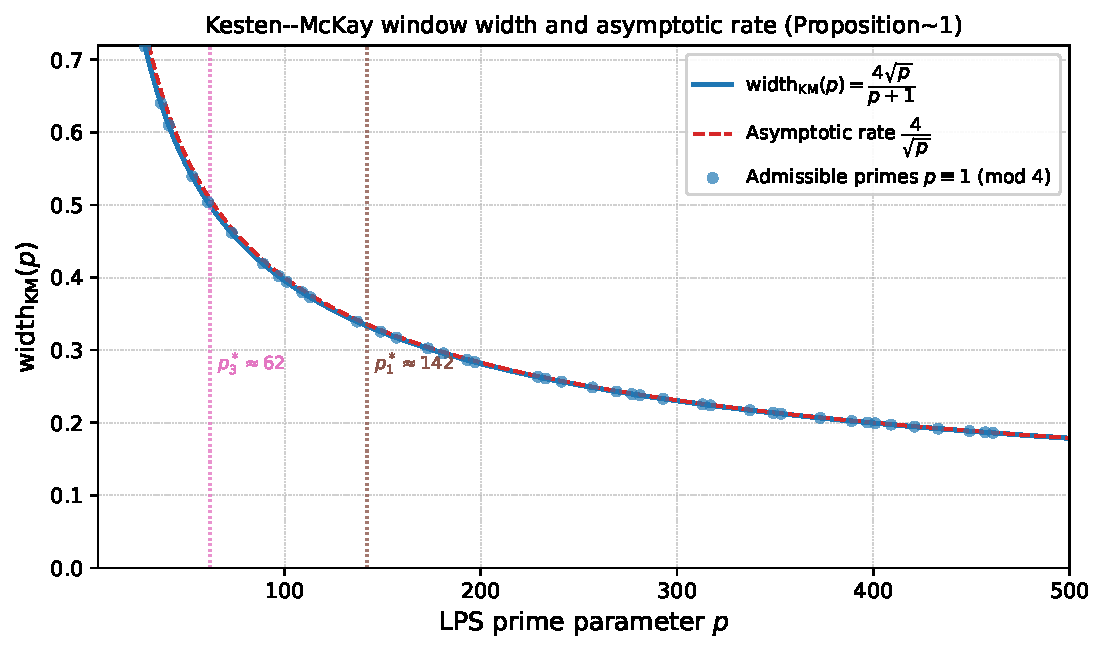
\includegraphics[width=0.82\textwidth]{../code/O1_fig2_KM_width}
      \caption{Kesten--McKay window width $\widthKM(p) = 4\sqrt{p}/(p+1)$ as a
      function of the LPS prime $p$ (solid blue), together with the asymptotic
      rate $4/\sqrt{p}$ (dashed red) and the admissible primes
        $p \equiv 1 \pmod{4}$ (dots).
        The two critical primes $p_3^* \approx 62$ and $p_1^* \approx 142$
        (Theorem~\ref{thm:exit_order}) are marked by vertical dotted lines.
        The width is a strictly decreasing function of $p$, confirming
        Proposition~\ref{prop:KM_contraction}.}
      \label{fig:KM_width}
    \end{figure}

  \subsection{Ordered exit of ADE levels}
    \label{subsec:exit_order}

    As the Kesten--McKay window narrows, the outer ADE levels will eventually
    exit the support.
    A level $\lADE{k} \neq 1$ exits at the critical prime $p_k^*$ defined by
    \begin{equation}
      \lADE{k} \;=\; \lambda_{\mathrm{sgn}}(p_k^*),
      \label{eq:exit_condition}
    \end{equation}
    where $\lambda_{\mathrm{sgn}}$ is $\lambda_+$ if $\lADE{k} > 1$ and
    $\lambda_-$ if $\lADE{k} < 1$.
    The geometry of this process is illustrated in Figure~\ref{fig:KM_contraction}.

    \begin{theorem}[ADE exit order]
      \label{thm:exit_order}
      For the $2I$ group with the order-5 generating set, the three ADE levels
      exit the Kesten--McKay support in the following order:
      \begin{enumerate}
        \item $\lADE{3} = 5/4$ exits the upper support edge at
        \begin{equation}
          p_3^* \;=\; \left(4 + \sqrt{15}\right)^2 \;\approx\; 62;
          \label{eq:p3_exit}
        \end{equation}
        \item $\lADE{1} = 5/6$ exits the lower support edge at
        \begin{equation}
          p_1^* \;=\; \left(6 + \sqrt{35}\right)^2 \;\approx\; 142;
          \label{eq:p1_exit}
        \end{equation}
        \item $\lADE{2} = 1$ never exits: it coincides with the midpoint of the
        support for every finite $p$.
      \end{enumerate}
      Hence the support-induced exit order is $\lADE{3}$ first, then $\lADE{1}$,
      with $\lADE{2}$ remaining inside the support for all finite $p$.
    \end{theorem}

    \begin{proof}
      \textit{Exit of $\lADE{3} = 5/4$.}
      A level $\lambda > 1$ exits the upper support edge when
      $\lambda = \lambda_+(p) = 1 + 2\sqrt{p}/(p+1)$, i.e., when
      \begin{equation}
        \frac{2\sqrt{p}}{p+1} \;=\; \lambda - 1.
        \label{eq:exit_eq}
      \end{equation}
      Setting $u = \sqrt{p}$, equation~\eqref{eq:exit_eq} becomes
      $(\lambda-1)u^2 - 2u + (\lambda-1) = 0$, with positive root
      \begin{equation}
        u \;=\; \frac{1 + \sqrt{1 - (\lambda-1)^2}}{\lambda - 1}.
        \label{eq:u_formula}
      \end{equation}
      For $\lADE{3} = 5/4$, one has $\lambda - 1 = 1/4$, giving
      $u = 4 + \sqrt{15}$, hence $p_3^* = (4 + \sqrt{15})^2 \approx 62$.

      \textit{Exit of $\lADE{1} = 5/6$.}
      Since the Kesten--McKay support is symmetric about $\lambda = 1$
      (cf.~\eqref{eq:support_symmetry}), a level $\lambda < 1$ exits the lower
      support edge at the same critical prime as the reflected level $2 - \lambda
      > 1$ exits the upper support edge.
      For $\lADE{1} = 5/6$, the reflected level is $2 - 5/6 = 7/6$, so
      $\lambda - 1 = 1/6$ in~\eqref{eq:exit_eq}, giving $u = 6 + \sqrt{35}$,
      hence $p_1^* = (6 + \sqrt{35})^2 \approx 142$.

      \textit{Non-exit of $\lADE{2} = 1$.}
      For every finite $p$, $\lambda_\pm(p) = 1 \pm 2\sqrt{p}/(p+1) \neq 1$,
      so the central level never coincides with a support edge.
    \end{proof}

    \begin{figure}[ht]
      \centering
      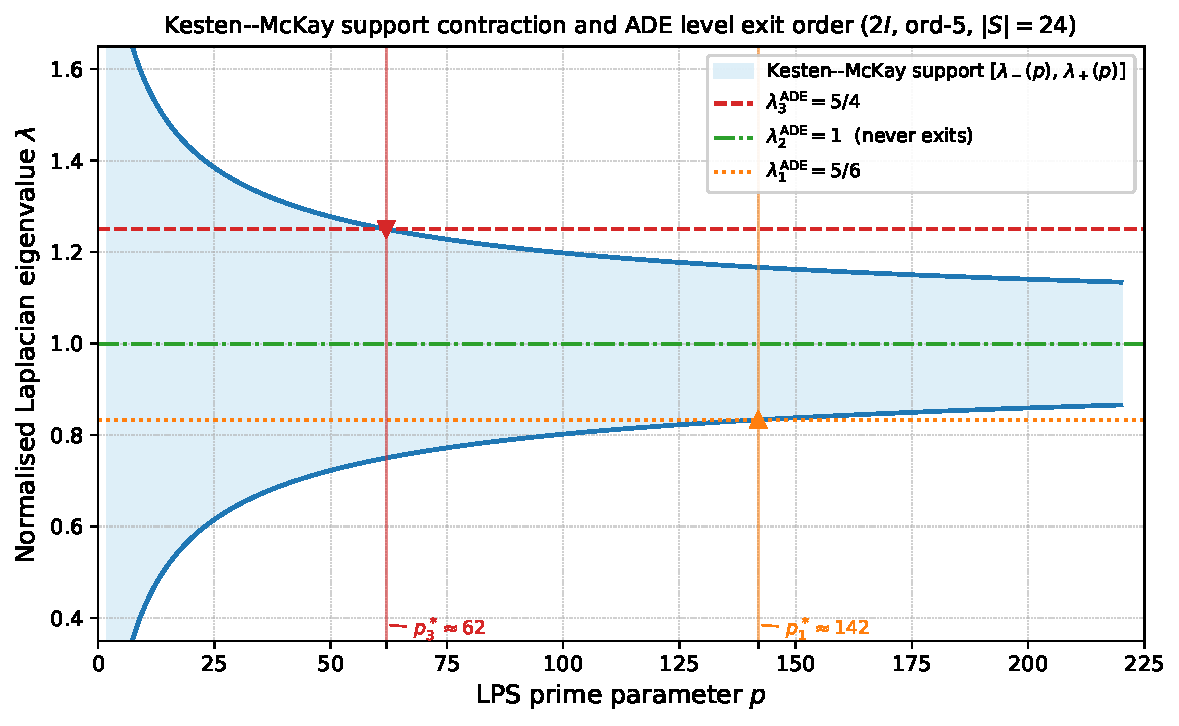
\includegraphics[width=0.88\textwidth]{../code/O1_fig1_KM_contraction}
      \caption{Kesten--McKay support contraction and ADE level exit order for the
        $2I$ group (ord-5 generating set, $|S|=24$).
        The shaded band is the Kesten--McKay support
        $[\lambda_-(p),\lambda_+(p)]$, which contracts symmetrically around the
        midpoint $\lambda=1$ as $p$ increases.
        The three horizontal lines are the fixed ADE levels
        $\lADE{1}=5/6$ (dotted orange), $\lADE{2}=1$ (dash-dot green),
        $\lADE{3}=5/4$ (dashed red).
        The downward triangle marks the exit of $\lADE{3}$ at
        $p_3^* = (4+\sqrt{15})^2 \approx 62$; the upward triangle marks the exit
        of $\lADE{1}$ at $p_1^* = (6+\sqrt{35})^2 \approx 142$.
        The central level $\lADE{2}=1$ never exits for any finite $p$.}
      \label{fig:KM_contraction}
    \end{figure}

    \begin{remark}[Independence from the growth law]
      \label{rem:universality}
      The ordering $p_3^* < p_1^*$ depends only on the positions of the ADE
      levels relative to the support midpoint, not on the function $p(n)$.
      For any variable-valence sequence eventually satisfying $p(n) > p_3^*$,
      the level $\lADE{3}$ has already exited the support; for $p(n) > p_1^*$,
      both outer levels have exited.
      The exit order is therefore a \emph{structural consequence} of the support
      geometry, universal across all admissible growth laws.
      Figure~\ref{fig:stab_ranks} confirms this numerically for three
      representative growth laws.
    \end{remark}

    \begin{figure}[ht]
      \centering
      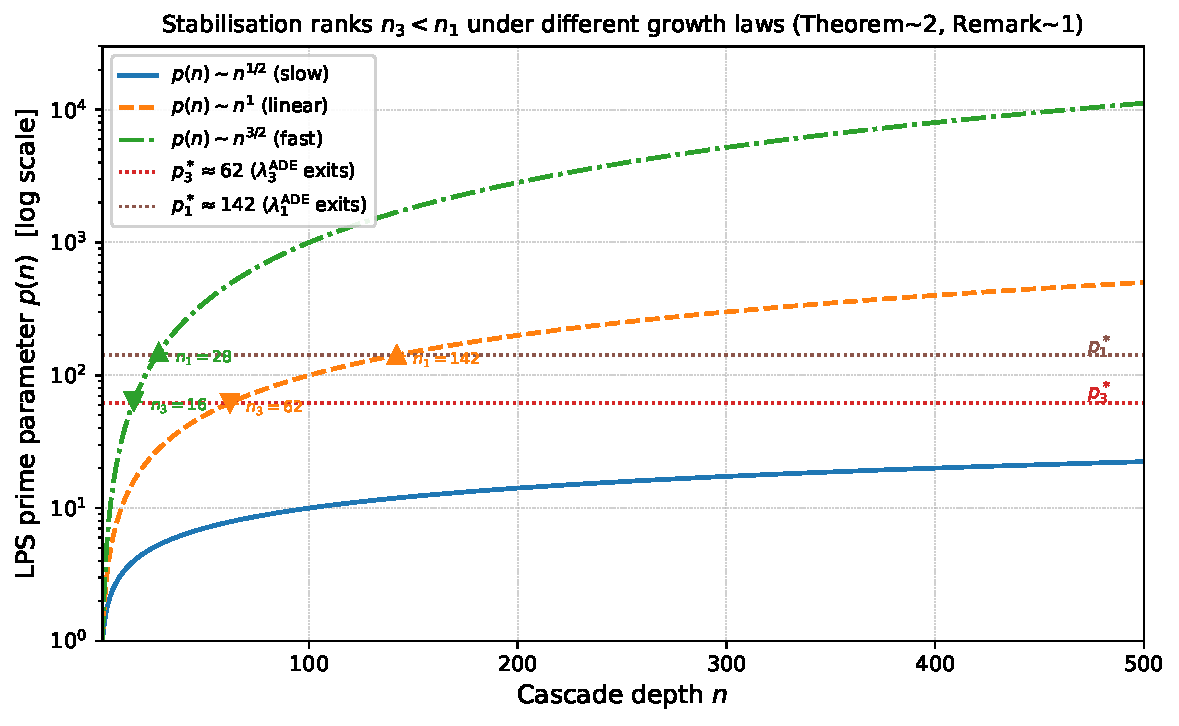
\includegraphics[width=0.82\textwidth]{../code/O1_fig3_stab_ranks}
      \caption{Stabilisation ranks $n_3 < n_1$ under three representative growth
      laws $p(n) \sim n^{1/2}$ (slow, solid blue), $p(n) \sim n$ (linear,
        dashed orange), and $p(n) \sim n^{3/2}$ (fast, dash-dot green), plotted
        on a logarithmic scale.
        Downward triangles mark $n_3 = \min\{n : p(n) \geq p_3^*\}$ and upward
        triangles mark $n_1 = \min\{n : p(n) \geq p_1^*\}$ for each law.
        In all cases $n_3 < n_1$, confirming that the ordering of stabilisation
        ranks is independent of the growth law (Remark~\ref{rem:universality}).}
      \label{fig:stab_ranks}
    \end{figure}

  \subsection{Restored lower-bound dynamics of projective resolution}
    \label{subsec:restored_dynamics}

    \begin{corollary}[Restored lower-bound dynamics]
      \label{cor:dynamics}
      Let $(G_n)$ be a variable-valence LPS sequence.
      Then the Ramanujan lower edge satisfies
      \begin{equation}
        \lambda_-(p(n)) \;=\; 1 - \frac{2\sqrt{p(n)}}{p(n)+1}
        \;\longrightarrow\; 1^-,
        \label{eq:lower_edge_to_1}
      \end{equation}
      and therefore the Cheeger lower bound on $\Lproj(n)$ obeys
      \begin{equation}
        \Lproj(n) \;\gtrsim\; \frac{\lambda_-(p(n))^2}{2}
        \;\longrightarrow\; \frac{1}{2}.
        \label{eq:lambda_proj_lower}
      \end{equation}
      In particular, the fixed-valence saturation plateau is structurally removed:
      $\Lproj(n)$ cannot remain frozen at the baseline associated with any fixed
      prime $p_0$.
    \end{corollary}

    \begin{proof}
      By~\eqref{eq:ramanujan_lower}, $\lambda_2(n) \geq \lambda_-(p(n))$.
      Since $p(n) \to \infty$, equation~\eqref{eq:KM_support_p} gives
      $\lambda_-(p(n)) \to 1^-$.
      The Cheeger lower bound~\eqref{eq:cheeger} then yields
      \[
        \Lproj(n) \;\gtrsim\; \frac{\lambda_2(n)^2}{2}
        \;\geq\; \frac{\lambda_-(p(n))^2}{2} \;\longrightarrow\; \frac{1}{2}.
      \]
      For any fixed $p_0$, one has $\lambda_-(p_0) < 1$, hence
      $\lambda_-(p_0)^2/2 < 1/2$.
      The lower bound on $\Lproj(n)$ therefore strictly exceeds the fixed-valence
      saturation value for all sufficiently large $n$.
    \end{proof}

    \begin{remark}[Physical interpretation]
  In the Cosmochrony framework, $p(n) \to \infty$ corresponds to an increase of the
  effective relational valence of the substrate along the cascade.
  Corollary~\ref{cor:dynamics} shows that this is the minimal structural
  condition preventing the relaxation cascade from freezing into a spectrally
  stationary regime.
    \end{remark}

  \section{Effective Mass Ordering Restoration}
  \label{sec:mass_ordering}


  We derive the effective mass ordering implied by the ADE exit order of
  Theorem~\ref{thm:exit_order} and show that it corrects the inversion
  identified in~\cite{Beau2026a5}.

  \subsection{Stabilisation by support exit}
    \label{subsec:stabilisation}

    A level $\lADE{k}$ that lies inside the Kesten--McKay support participates in
    the relaxation dynamics.
    Once $p$ exceeds the critical value $p_k^*$, the level exits the support and
    is \emph{stabilised}: it no longer participates in the evolving spectral
    dynamics and its effective mass is frozen at the cascade rank where
    $p(n) \approx p_k^*$.

    \begin{definition}[Stabilisation rank]
      \label{def:stabilisation_rank}
      The \emph{stabilisation rank} of the level $\lADE{k}$ along a
      variable-valence LPS sequence $(G_n)$ is
      \begin{equation}
        n_k \;:=\; \min\bigl\{\,n \geq 1 : p(n) \geq p_k^*\,\bigr\},
        \label{eq:stab_rank}
      \end{equation}
      where $p_k^*$ is the critical prime of Theorem~\ref{thm:exit_order}.
    \end{definition}

    The ordering of stabilisation ranks is determined solely by the ordering of
    the critical primes: since $p_3^* < p_1^*$, any variable-valence sequence
    with $p(n) \to \infty$ satisfies $n_3 < n_1$, independently of the growth
    law $p(n)$.

  \subsection{Effective mass ordering}
    \label{subsec:mass_from_exit}

    We assign effective masses according to stabilisation rank: a level that
    stabilises earlier acquires a higher effective mass, following the assignment
    principle of~\cite{Beau2026a4,Beau2026a5}.
    From Theorem~\ref{thm:exit_order} and the ordering $p_3^* < p_1^*$:
    \begin{equation}
      M_3 \;>\; M_1 \;>\; M_2,
      \label{eq:mass_ordering}
    \end{equation}
    where $M_k$ denotes the effective mass associated with $\lADE{k}$.

  \subsection{Correction of the fixed-valence inversion}
    \label{subsec:inversion_correction}

    Under the fixed-valence saturation mechanism of~\cite{Beau2026a5}, the
    effective mass ordering was governed by $\FKM(\lADE{k})$, monotone increasing
    in $\lADE{k}$, producing $M_1 < M_2 < M_3$ and inverting the ordering
    required by~\cite{Beau2026a4}.

    In the variable-valence regime, the ordering~\eqref{eq:mass_ordering} is
    generated by the support-exit geometry: the ordering mechanism is now geometric
    (position of a fixed level relative to a contracting support boundary) rather
    than analytic (monotonicity of the cumulative density).
    This is a qualitative structural change that corrects the fixed-valence
    inversion without introducing any additional dynamical hypothesis.

    The level-to-generation map is not established from first principles within
    this paper and is therefore left open.

    \begin{remark}[Compatible physical interpretation]
  If one identifies $\lADE{3} = 5/4$, which stabilises first and acquires the
  highest effective mass, with the heaviest charged-lepton generation, then
  the ordering~\eqref{eq:mass_ordering} is compatible with the observed
  hierarchy $m_\tau > m_\mu > m_e$.
  Establishing this identification from first principles remains open.
    \end{remark}

    \begin{remark}[Structural universality]
      \label{rem:universality_mass}
      By Remark~\ref{rem:universality}, the effective mass ordering
      \eqref{eq:mass_ordering} holds for any variable-valence LPS sequence
      eventually surpassing $p_1^* \approx 142$, independently of the growth
      law $p(n)$.
    \end{remark}

  \section{Amplitude Problem: Partial Resolution and Residual Gap}
  \label{sec:amplitude}


  Having shown that the variable-valence regime corrects the effective mass
  ordering inversion, we examine how much of the amplitude problem it resolves
  and where a residual gap remains.

  \subsection{What the variable-valence mechanism provides}
    \label{subsec:what_is_gained}

    In the fixed-valence regime, the effective mass ratio was~\cite{Beau2026a5}:
    \begin{equation}
      \frac{M_i}{M_j} \;=\;
      \frac{\FKM(\lADE{i})}{\FKM(\lADE{j})}
      \cdot \frac{\dim \rho_{\lambda_j}}{\dim \rho_{\lambda_i}},
      \label{eq:mass_ratio_fixed}
    \end{equation}
    with all levels evaluated in a single Kesten--McKay window at fixed $p$,
    yielding ratios in $[0.10, 2.2]$.

    In the variable-valence regime, each generation stabilises at a distinct
    rank $n_k$ where $p(n_k) \approx p_k^*$, giving:
    \begin{equation}
      \frac{M_i}{M_j} \;\simeq\;
      \frac{\FKM(\lADE{i};\,p(n_i))}{\FKM(\lADE{j};\,p(n_j))}
      \cdot \frac{\dim \rho_{\lambda_j}}{\dim \rho_{\lambda_i}},
      \label{eq:mass_ratio_variable}
    \end{equation}
    with numerator and denominator evaluated at different primes.
    Since the cumulative spectral mass near a support edge becomes parametrically
    small, support-exit separation across distinct stabilisation ranks can in
    principle generate stronger inter-generational suppression than the
    fixed-valence formula~\eqref{eq:mass_ratio_fixed} allows.

  \subsection{Residual amplitude gap}
    \label{subsec:amplitude_gap}

    Reaching the observed hierarchy $m_e/m_\tau \approx 3 \times 10^{-4}$
    requires ratios of order $10^{-4}$ from~\eqref{eq:mass_ratio_variable},
    which demands additional structure beyond direction (O1) alone:
    \begin{enumerate}
      \item a hierarchical cascade operating recursively across $L \geq 3$ nested
      levels, with per-level ratio $r$ accumulating as $r^L$ (direction (O2)
      of~\cite{Beau2026a5}); or
      \item a sub-linear energy-rank relation $E_n \propto n^{-\alpha}$ with
      $\alpha < 1$ (direction (O3) of~\cite{Beau2026a5}).
    \end{enumerate}
    A complete quantitative resolution requires combining direction (O1) with (O2)
    or (O3), and is deferred to subsequent work.

    \begin{remark}[Scope of the present result]
      \label{rem:scope}
      This paper establishes that the effective mass ordering inversion is
      corrected by a structural mechanism requiring no additional dynamical
      hypothesis, and that the fixed-valence saturation plateau is removed.
      The amplitude gap of order $10^{-4}$--$10^{-5}$ is not closed here, but
      the structural obstruction to closing it is removed.
    \end{remark}

  \section{Physical Interpretation in the Cosmochrony Framework}
  \label{sec:physical}

  \subsection{Relational valence and the cascade}
    \label{subsec:valence_cascade}

    In the Cosmochrony framework~\cite{cosmochrony}, the relaxation graph $G_n$ encodes
    the relational connectivity of the substrate at cascade depth $n$.
    The valence $d(n) = p(n) + 1$ measures the degree of connectivity at that
    depth.

    The fixed-valence regime corresponds to a substrate whose relational
    connectivity does not evolve along the cascade: the Kesten--McKay support is
    static, $\Lproj(n)$ saturates, and no inter-generational hierarchy can be
    generated.

    The variable-valence regime $p(n) \to \infty$ corresponds to a substrate
    whose effective relational connectivity increases along the cascade.
    Proposition~\ref{prop:KM_contraction} shows that this causes the Kesten--McKay
    support to contract progressively around $\lambda = 1$, and
    Corollary~\ref{cor:dynamics} shows that the fixed-valence saturation plateau
    is structurally removed.

  \subsection{Support contraction as spectral stratification}
    \label{subsec:stratification}

    The Kesten--McKay contraction is the spectral mechanism that generates
    stratification in the variable-valence regime.
    As the support narrows, the outer ADE levels exit in a fixed order
    (Theorem~\ref{thm:exit_order}), each exit corresponding to the stabilisation
    of one generation.

    This mechanism is structurally distinct from the fixed-valence saturation
    of~\cite{Beau2026a5}, where all three levels remained simultaneously inside
    the support and their ordering was governed by cumulative spectral mass alone.
    In the variable-valence regime, the ordering is governed by the geometry of
    a moving support boundary relative to fixed spectral landmarks.
    The two mechanisms are complementary: support-exit ordering (present paper)
    and cumulative-mass ordering~\cite{Beau2026a5} coexist in the full cascade,
    with support-exit ordering dominating when $p(n)$ grows with $n$.

  \subsection{Minimal structural requirement}
    \label{subsec:minimal}

    The variable-valence LPS family is the minimal extension of the fixed-valence
    LPS family that simultaneously:
    \begin{enumerate}
      \item preserves the Ramanujan property at each step, so that the spectral
      admissibility framework of~\cite{Beau2026a1} remains valid;
      \item causes the Kesten--McKay support to contract
      (Proposition~\ref{prop:KM_contraction}); and
      \item generates a non-trivial ADE exit order
      (Theorem~\ref{thm:exit_order}).
    \end{enumerate}
    Any relaxation graph family satisfying these three conditions produces the
    same qualitative result.
    The LPS family is used here because it provides an explicit, analytically
    tractable realisation.

  \section{Conclusion}
  \label{sec:conclusion}


  This paper revisits the saturation mechanism identified in~\cite{Beau2026a5}
  and shows that it is not a fundamental property of the relational substrate
  but a consequence of holding the LPS parameter $p$ constant.

  \subsection{Summary of results}
    \label{subsec:summary}

    Three results were established.

    The first (Proposition~\ref{prop:KM_contraction}) is that the Kesten--McKay
    window width $4\sqrt{p(n)}/(p(n)+1)$ converges to zero along any
    variable-valence LPS sequence, with both support edges approaching the midpoint
    $\lambda = 1$ at rate $2/\sqrt{p(n)}$.
    This is the fundamental spectral mechanism of the variable-valence regime.

    The second (Theorem~\ref{thm:exit_order}) is that the three ADE eigenvalue
    levels exit the contracting support in a fixed, growth-law-independent order:
    $\lADE{3} = 5/4$ exits first at $p_3^* = (4+\sqrt{15})^2 \approx 62$,
    $\lADE{1} = 5/6$ exits second at $p_1^* = (6+\sqrt{35})^2 \approx 142$, and
    $\lADE{2} = 1$ never exits for any finite $p$.
    The exit order is a structural consequence of the positions of the ADE levels
    relative to the contracting support boundary.

    The third (Corollary~\ref{cor:dynamics} and Section~\ref{sec:mass_ordering})
    is that the effective mass ordering $M_3 > M_1 > M_2$ follows directly from
    the exit order, correcting the inversion $M_1 < M_2 < M_3$ of~\cite{Beau2026a5}
    by a geometric mechanism requiring no additional dynamical hypothesis.

    These three results establish that:
    \begin{enumerate}
      \item[(i)] the fixed-valence saturation plateau of~\cite{Beau2026a5} is an
      artefact of holding $p$ constant;
      \item[(ii)] allowing $p(n) \to \infty$ restores a non-trivial dynamical
      regime in which ADE levels exit the Kesten--McKay support in a
      fixed order; and
      \item[(iii)] this minimal structural modification corrects the effective mass
      ordering inversion without introducing additional dynamical
      assumptions.
    \end{enumerate}

  \subsection{Open directions}
    \label{subsec:open}

    Three directions remain open.

    \paragraph{Amplitude problem.}
      The variable-valence mechanism decouples the stabilisation ranks of the three
      generations and allows inter-generational suppression stronger than the
      fixed-valence formula, but reaching the observed hierarchy
      $m_e/m_\tau \approx 3 \times 10^{-4}$ requires combining direction (O1) with
      the hierarchical cascade of direction (O2) or the sub-linear energy-rank
      relation of direction (O3) of~\cite{Beau2026a5}.

    \paragraph{Level-to-generation map.}
      The effective mass ordering $M_3 > M_1 > M_2$ is a structural result;
      its identification with the charged-lepton hierarchy $m_\tau > m_\mu > m_e$
      requires a first-principles derivation of the level-to-generation
      correspondence from the construction of~\cite{Beau2026a4}.

    \paragraph{Upper bound on $\Lproj(n)$.}
      The present analysis relies only on the Ramanujan lower bound through the
      edge $\lambda_-(p(n))$.
      A refined control of the upper Cheeger bound $\lambda_2(n)$
      in~\eqref{eq:cheeger} in the variable-valence regime could strengthen the
      dynamical interpretation of $\Lproj(n)$ and remains an open problem.

      \clearpage
      \bibliographystyle{plain}
      \bibliography{cosmochrony-bibliography}

\end{document}
